\documentclass[letterpaper, 12pt]{math}

\usepackage{tikz}

\title{Multivariable and Vector Calculus}
\author{Alvin Lin}
\date{August 2017 - December 2017}

\begin{document}

\maketitle

\section*{Functions of Several Variables}
A function of a single variable:
\begin{center}
  \begin{tikzpicture}
    \draw (0,0) -- node[below] {x} (2,0) -- node[right] {x} (2,2) --
      (0,2) -- (0,0);
  \end{tikzpicture}
\end{center}
\[ A(x) = x^2 \]
A function of two variables:
\begin{center}
  \begin{tikzpicture}
    \draw (0,0) -- node[below] {x} (4,0) -- node[right] {y} (4,2) --
      (0,2) -- (0,0);
  \end{tikzpicture}
\end{center}
\[ A(x,y) = xy \]
Even for functions of many variables, they still have properties such as domain
and range.
\[ f(x,y) = \frac{1}{\sqrt{1-x^2-y^2}} \]
Domain:
\[ 1-x^2-y^2 > 0 \therefore x^2+y^2 < 1 \]
Range:
\[ [1,\infty) \]

\subsubsection*{Example}
Find the domain of the function:
\[ f(x,y) = \frac{\ln(2-x)}{\sqrt{x-3y}} \]
\begin{align*}
  2-x &> 0 \\
  &\equiv x < 2\\
  x-3y &> 0 \\
  &\equiv y < \frac{x}{3}
\end{align*}
\begin{center}
  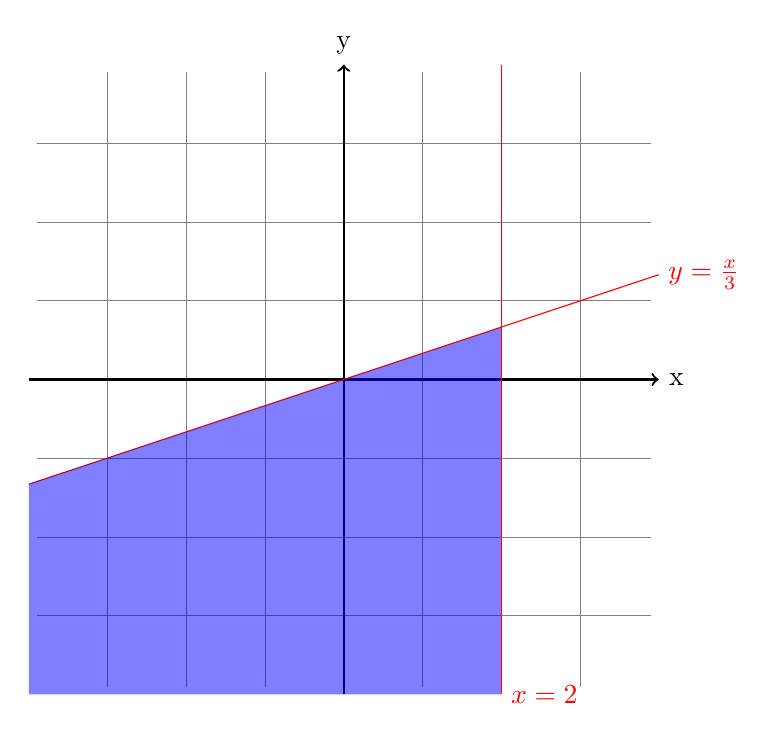
\begin{tikzpicture}
    \draw[step=1cm,gray,very thin] (-3.9,-3.9) grid (3.9,3.9);
    \draw[thick,->] (-4,0) -- (4,0) node[right] {x};
    \draw[thick,->] (0,-4) -- (0,4) node[above] {y};
    \draw[red] (2,4) -- (2,-4) node[right] {\( x = 2 \)};
    \draw[red] (-4,-1.33) -- (4,1.33) node[right] {\( y = \frac{x}{3} \)};
    \fill[opacity=0.5,blue] (-4,-1.33) -- (2,0.66) -- (2,-4) -- (-4,-4) --
      cycle;
  \end{tikzpicture}
\end{center}

\section*{Limits}

\subsubsection*{Example}
\[ \lim_{(x,y)\to(2,1)}\frac{xy}{x^2+2y^2} = \frac{1}{3} \]

\subsubsection*{Example}
\begin{align*}
  \lim_{(x,y)\to(0,0)}\frac{x^2+y^2}{\sqrt{1-x^2+y^2}-1} &=
    \lim_{(x,y)\to(0,0)}\frac{(x^2+y^2)(\sqrt{1-x^2-y^2+1})}
    {(\sqrt{1-x^2-y^2}-1)(\sqrt{1-x^2-y^2}+1)} \\
  &= \lim_{(x,y)\to(0,0)}\frac{(x^2+y^2)(\sqrt{1-x^2-y^2+1})}
    {1-x^2-y^2+1} \\
  &= -2
\end{align*}

\subsection*{Definition}
\[ lim_{(x,y)\to(x_{\circ},y_{\circ})} = L \]
is defined as for every \( \epsilon > 0 \) there exists \( \delta > 0 \) such
that \( |f(x,y)-L| < \epsilon \) if \( dist((x,y),(x_{\circ},y_{\circ}))
< \delta \). Notice that if:
\[ \lim_{(x,y)\to(x_{\circ},y_{\circ})}f(x,y) = L \quad\text{ and }\quad
  \lim_{(x,y)\to(x_{\circ},y_{\circ})}g(x,) = M \]
Then:
\[ \lim_{(x,y)\to(x_{\circ},y_{\circ})}\frac{f(x,y)}{g(x,y)} = \frac{L}{M} \]

\subsection*{Theorem}
If:
\[ \lim_{(x,y)\to(x_{\circ},y_{\circ})}f(x,y)\text{ on }C_1 \ne
  \lim_{(x,y)\to(x_{\circ},y_{\circ})}f(x,y)\text{ on }C_1 \]
Then \( \lim_{(x,y)\to(x_{\circ},y_{\circ})}f(x,y)\text{ on }C_1 \) does not
exist.

\subsubsection*{Example}
\[ \lim_{(x,y)\to(0,0)}\frac{xy}{x^2+2y^2} = \lim_{(x,y)\to(0,0)}\frac{0}{x^2} =
  \lim_{(x,y)\to(0,0)}\frac{0}{2y^2} = 0 \]
Inconclusive according to the theorem above. Take \( y = kx \):
\[ \lim_{(x,y)\to(x_{\circ},y_{\circ})}\frac{xkx}{x^2+2kx^2} =
  \lim_{(x,y)\to(x_{\circ},y_{\circ})}\frac{k}{1+2k} = \frac{k}{1+2k} \]
The original limit does not exist.

\subsubsection*{Example}
\[ \lim_{(x,y)\to(0,0)}\frac{x^2y}{x^2+2y^2} \]
Take \( y = kx \):
\[ \lim_{x\to0}\frac{x^2kx}{x^2+2k^2x^2} = \lim_{x\to0}\frac{kx}{1+2k^2} = 0 \]
Take \( y = kx^2 \):
\[ \lim_{x\to0}\frac{x^2kx^2}{x^2+2k^2x^4} = \lim_{x\to0}\frac{kx^2}{1+2k^2x^2}
  = 0 \]
By the Squeeze Theorem:
\[ \lim_{(x,y)\to(0,0)}0 \le \lim_{(x,y)\to(0,0)}\frac{x^2y}{x^2+2y^2} \le
  \lim_{(x,y)\to(0,0)}y \]
We can conclude that \( \lim_{(x,y)\to(0,0)}\frac{x^2y}{x^2+2y^2} = 0 \).

\section*{Partial Derivatives}
\[ \lim_{h\to0}\frac{f(x+h,h_{\circ})-f(x,y_{\circ})}{h} =
  \pdiff{f}{x}(x,y_{\circ}) \]
Examples:
\begin{align*}
  \pdiff{}{y}(x^2y^3-x^2+xy) &= x^23y^2+x \\
  \pdiff{}{x}(x^2y^3-x^2+xy) &= y^32x-2x+y \\
  \pdiff{}{x}(x^y) &= yx^{y-1} \\
  \pdiff{}{y}(x^y) &= x^y\ln(x)
\end{align*}
Extensions:
\[ \pdiff{}{x}\pdiff{f}{x} = \frac{\partial^2{f}}{\partial{x^2}} \]
\[ \pdiff{}{y}\pdiff{f}{y} = \frac{\partial^2{f}}{\partial{y^2}} \]
\[ \pdiff{}{y}\pdiff{f}{x} = \frac{\partial^2{f}}{\partial{y}\partial{x}} \]
\[ \pdiff{}{x}\pdiff{f}{y} = \frac{\partial^2{f}}{\partial{x}\partial{y}} \]

\subsection*{Clairaut's Theorem}
If \( \frac{\partial^2{f}}{\partial{x}\partial{y}} \) and \(
\frac{\partial^2{f}}{\partial{y}\partial{x}} \) are continuous in some
neighborhood of \( (x_{\circ},y_{\circ}) \), then:
\[ \frac{\partial^2}{\partial{x}\partial{y}}(x_{\circ},y_{\circ}) =
  \frac{\partial^2}{\partial{y}\partial{x}}(x_{\circ},y_{\circ}) \]

\begin{center}
  You can find all my notes at \url{http://omgimanerd.tech/notes}. If you have
  any questions, comments, or concerns, please contact me at
  alvin@omgimanerd.tech
\end{center}

\end{document}
